%-------------------------------------------------------------------------------
% LATEX TEMPLATE ARTIKEL
%-------------------------------------------------------------------------------
% Dit template is voor gebruik door studenten van de de bacheloropleiding 
% Informatica van de Universiteit van Amsterdam.
% Voor informatie over schrijfvaardigheden, zie 
%                               https://practicumav.nl/schrijven/index.html
%
%-------------------------------------------------------------------------------
%	PACKAGES EN DOCUMENT CONFIGURATIE
%-------------------------------------------------------------------------------

\documentclass{uva-inf-article}
\usepackage[english]{babel}
\usepackage{tikz}
\usepackage{pdflscape}
\usepackage{todonotes}

\usepackage[style=authoryear-comp]{biblatex}
\addbibresource{references.bib}

%-------------------------------------------------------------------------------
%	GEGEVENS VOOR IN DE TITEL, HEADER EN FOOTER
%-------------------------------------------------------------------------------

% Geef je artikel een logische titel die de inhoud dekt.
\title{Blender Documentation}

% Vul de naam van de opdracht in zoals gegeven door de docent en het type 
% opdracht, bijvoorbeeld 'technisch rapport' of 'essay'.
% \assignment{}
% \assignmenttype{}

% Vul de volledige namen van alle auteurs in en de corresponderende UvAnetID's.
\authors{Jari Andersen}
% \uvanetids{}

% Vul de naam van je tutor, begeleider (mentor), of docent / vakcoördinator in.
% Vermeld in ieder geval de naam van diegene die het artikel nakijkt!
% \tutor{}
% \mentor{}
% \docent{}

% Vul hier de naam van je tutorgroep, werkgroep, of practicumgroep in.
% \group{SignLab, VisualisationLab}

% Vul de naam van de cursus in en de cursuscode, te vinden op o.a. DataNose.
% \course{}
% \courseid{}

% Dit is de datum die op het document komt te staan. Standaard is dat vandaag.
\date{\today}

%-------------------------------------------------------------------------------
%	VOORPAGINA 
%-------------------------------------------------------------------------------

\begin{document}
\maketitle
\tableofcontents
\newpage
%-------------------------------------------------------------------------------
%	INHOUDSOPGAVE EN ABSTRACT
%-------------------------------------------------------------------------------
% Niet toevoegen bij een kort artikel, zeg minder dan 10 pagina's!

%TC:ignore
%\tableofcontents
%\begin{abstract}
%\end{abstract}
%TC:endignore

%-------------------------------------------------------------------------------
%	INHOUD
%-------------------------------------------------------------------------------
% Hanteer bij benadering IMRAD: Introduction, Method, Results, Discussion.
\section{Introduction}
Blender is a powerful and versatile open-source 3D creation suite that supports the entirety of the 3D pipeline, including modeling, rigging, animation, simulation, rendering, compositing, and motion tracking. In this document, we will explore various aspects of using Blender, and the integration with Unreal Engine.

The content is structured to guide users through practical steps and troubleshooting tips


\section{Importing from Unreal Engine export}
When exporting through Unreal Engine, the engine uses its own coordinate system. This system does not match Blender's coordinate system and will therefore orientate the bones wrongly when using the default import settings in blender (resulting in figure \ref{fig:wrongimport}). In order to get the correct orientations use the options in figure \ref{fig:correctimportsettings}.

\begin{figure}[hbt!]
    \centering
    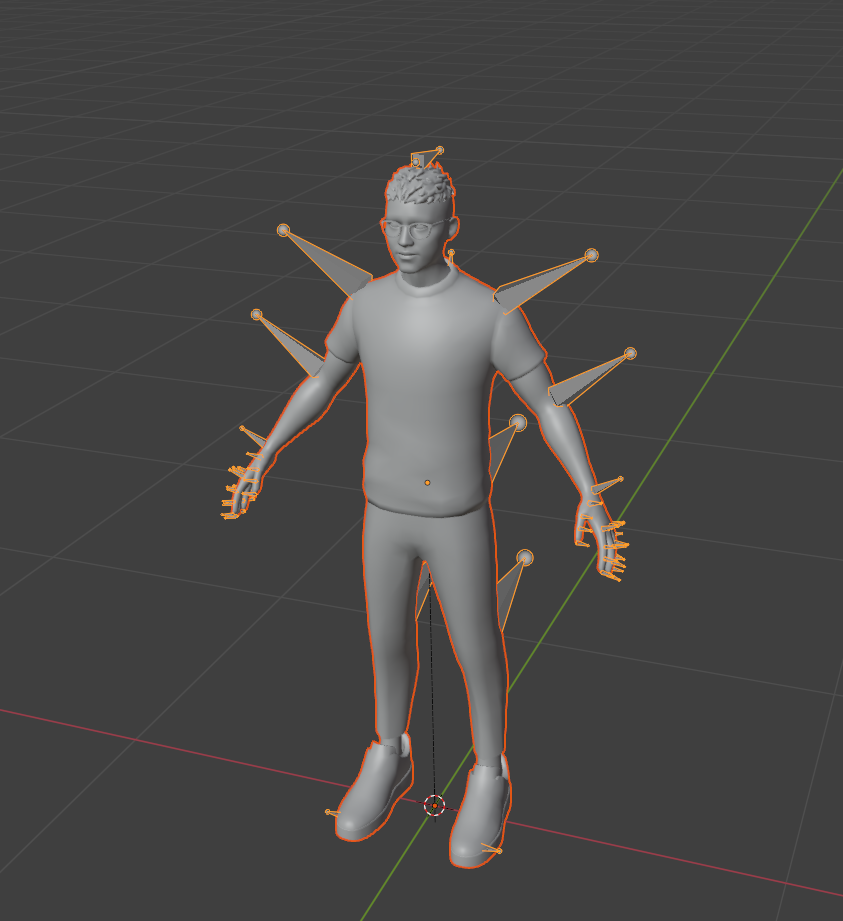
\includegraphics[width=0.5\textwidth]{imgs/wrongorientation.png}
    \caption{Blender default import settings for an Unreal Engine exported avatar.}
    \label{fig:wrongimport}
\end{figure}

\begin{figure}[hbt!]
    \centering
    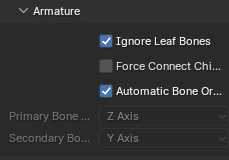
\includegraphics[width=0.5\textwidth]{imgs/importsettings.png}
    \caption{Blender import settings for an Unreal Engine exported avatar resulting in correct bone orientation.}
    \label{fig:correctimportsettings}
\end{figure}

\section{Rigging Techniques in Blender}
\subsection{Modifying the rest pose}
Modifying the rest pose can be important due to various reasons. One might want to edit this because of the StretchSense software where a T-pose is required (see section \ref{section:stretchsense}). In my efforts to learning this system I came across 2 issues that will be discussed in this section.

\subsubsection{Mirror mode}
Firstly, we need to rotate the bones into the new pose (for example a T-pose). We do not want to rotate the left and right side individually, that would take twice as long as rotating 1 side of the avatar and simply mirroring this rotation onto the other side. Figure \ref{fig:mirrorOption} shows this option to mirror bone rotation in the Pose Mode view.
If you don't turn on automatic bone orientation in the armature import settings (figure \ref{fig:correctimportsettings}) or don't make sure the bone axis is aligned with the correct axis in blender, the bone rotation will not be mirrored correctly resulting in figure \ref{fig:mirrorWrong}. Lastly, if none of these options worked, we can recalculate the ``bone roll" in Edit Mode (see figure \ref{fig:recalcboneroll}). We recalculate based on where the avatar is facing.
\begin{figure}[hbt!]
    \centering
    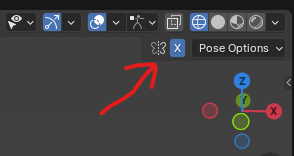
\includegraphics[width=0.5\textwidth]{imgs/mirrormode.png}
    \caption{Blender Pose Mode - mirror option}
    \label{fig:mirrorOption}
\end{figure}

\begin{figure}[hbt!]
    \centering
    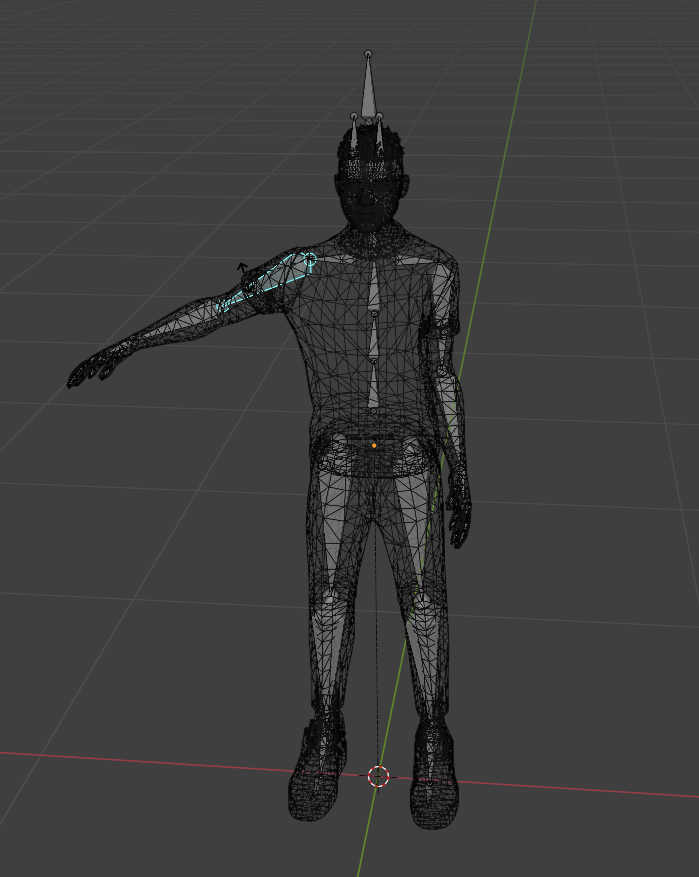
\includegraphics[width=0.5\textwidth]{imgs/wrongMirrorMode.png}
    \caption{Blender Pose Mode - wrong mirror}
    \label{fig:mirrorWrong}
\end{figure}
\begin{figure}[hbt!]
    \centering
    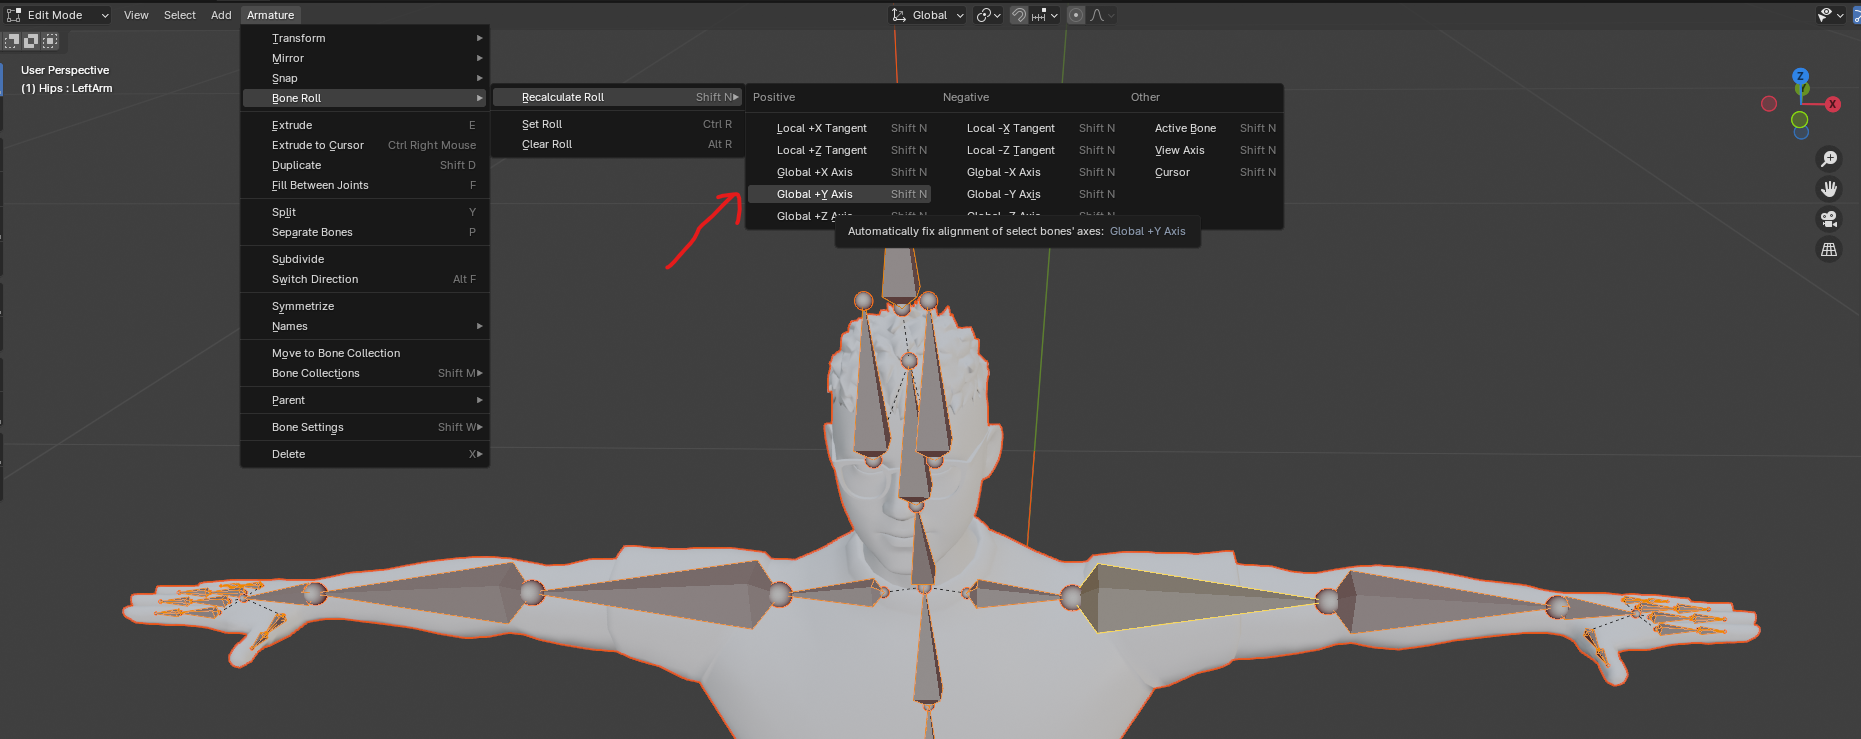
\includegraphics[width=1\textwidth]{imgs/resetRoll.png}
    \caption{Blender Edit Mode - the recalculate bone roll option}
    \label{fig:recalcboneroll}
\end{figure}

\subsubsection{Applying the new pose - Blender method}\label{poseApplyBlender}
After putting the avatar into the desired pose, we want to make this the resting pose. This allows us to export the avatar and have it retain that pose across all 3D software that we use. Logically, we would go into Pose Mode and ``Apply Pose as Rest Pose". However, this results in the mesh getting detached from the skeleton and only the skeleton retaining the rest pose (figure \ref{fig:restPoseWrong}).
\begin{figure}[hbt!]
    \centering
    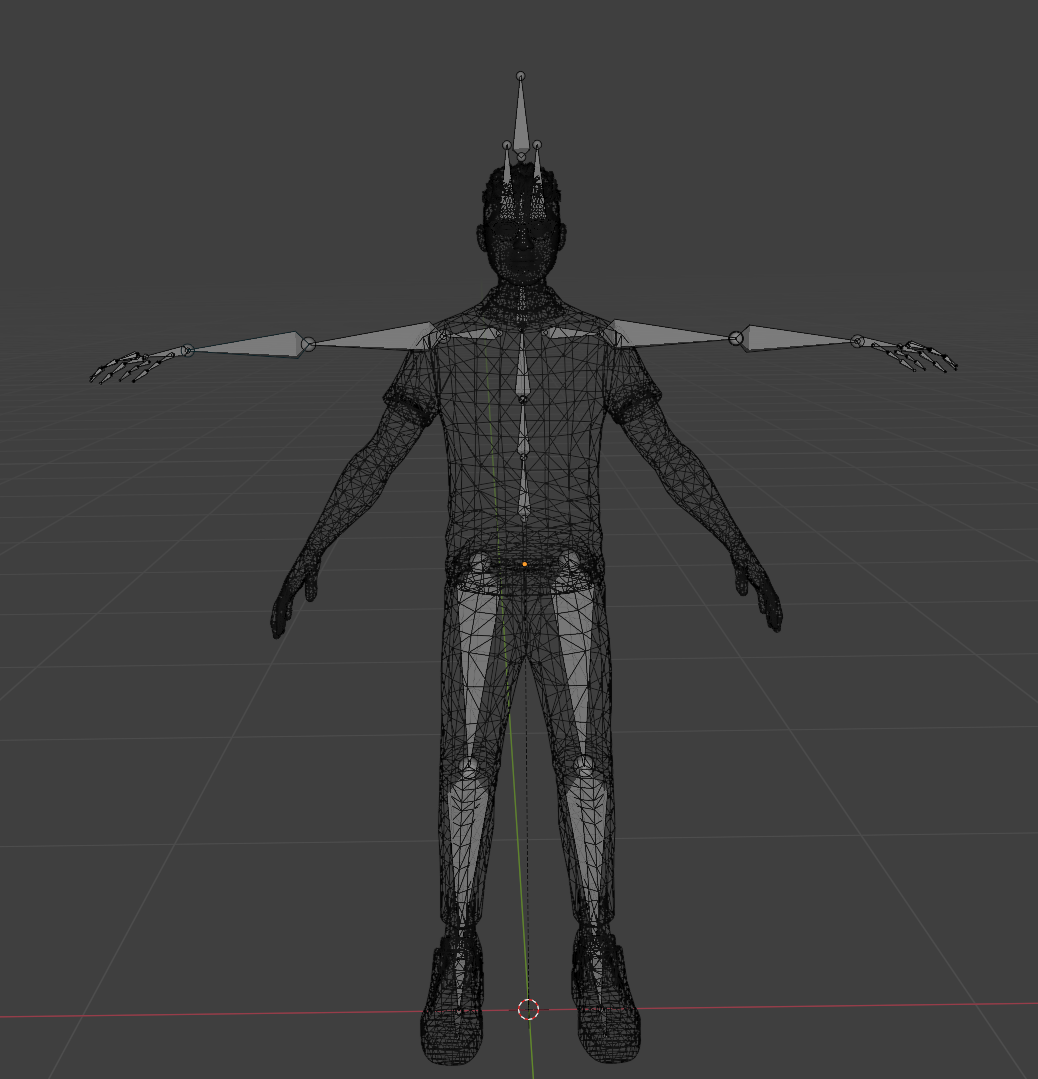
\includegraphics[width=0.5\textwidth]{imgs/wrongRest.png}
    \caption{Blender Pose Mode - detached mesh from rest pose}
    \label{fig:restPoseWrong}
\end{figure}
In order to circumvent this problem, we follow the steps in this blog: \href{https://nixart.wordpress.com/2013/03/28/modifying-the-rest-pose-in-blender/}{Modifying the Rest Pose in Blender}.
Which I will repeat now:
\begin{enumerate}
    \item Select your armature and go in “Pose Mode”.
    \item Pose your object in your new rest pose.
    \item Go in “Object Mode” and select your deformed object.
    \item In the object’s “Object Modifiers” stack, copy the “Armature Modifier” by pressing the “Copy” button. You should have two “Armature Modifiers”, one above the other in the stack, with the same parameters. This will deform your object twice, but it is ok. If you go in “Edit Mode”, you will see that the mesh has been deformed in your new rest pose.
    \item Apply the first “Armature Modifier” (the top one), but keep the bottom one. The latter will replace the old “Armature Modifier” and will allow to pose your object with respect to your new rest pose. At this point, the object will still be deformed twice. That is because we need to apply the current pose as the new rest pose.
    \item Select your armature and go in “Pose Mode”.
    \item “Apply Pose as Rest Pose” in the “Pose” menu. This will clear the double deformation and put your object in your new rest pose.
\end{enumerate}

Because I had trouble finding the armature modifier location, I will explain where it is. In Object Mode, we select the mesh (NOT the skeleton) and then it can be found in figure \ref{fig:armMod}.
\begin{figure}[hbt!]
    \centering
    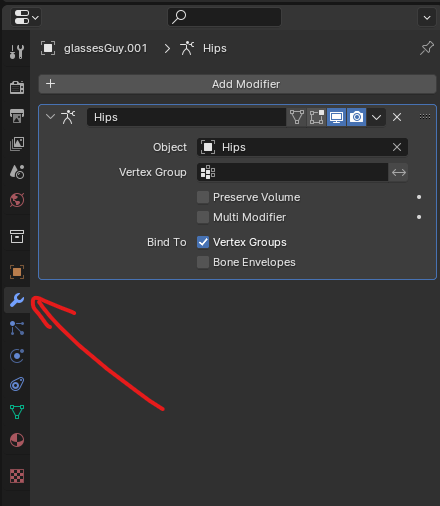
\includegraphics[width=0.5\textwidth]{imgs/Armature Modifier Location.png}
    \caption{Blender Object Mode - with the mesh selected, this is the location of the armature modifier}
    \label{fig:armMod}
\end{figure}

\subsubsection{Applying the new pose - plugin method}
Because the steps in section \ref{poseApplyBlender} are a hastle to go through everytime. I've looked up a different quicker method. Using the \href{https://github.com/cgvirus/Simple-Retarget-Tool-Blender}{Simple-Retarget-Tool-Blender} by cgvirus, we can apply the pose with only one button. After posing your avatar, select any part of the armature of the avatar and click the ``set rest pose with objects" (see figure \ref{fig:restPoseQuick}). And done is peter.

\begin{figure}[hbt!]
    \centering
    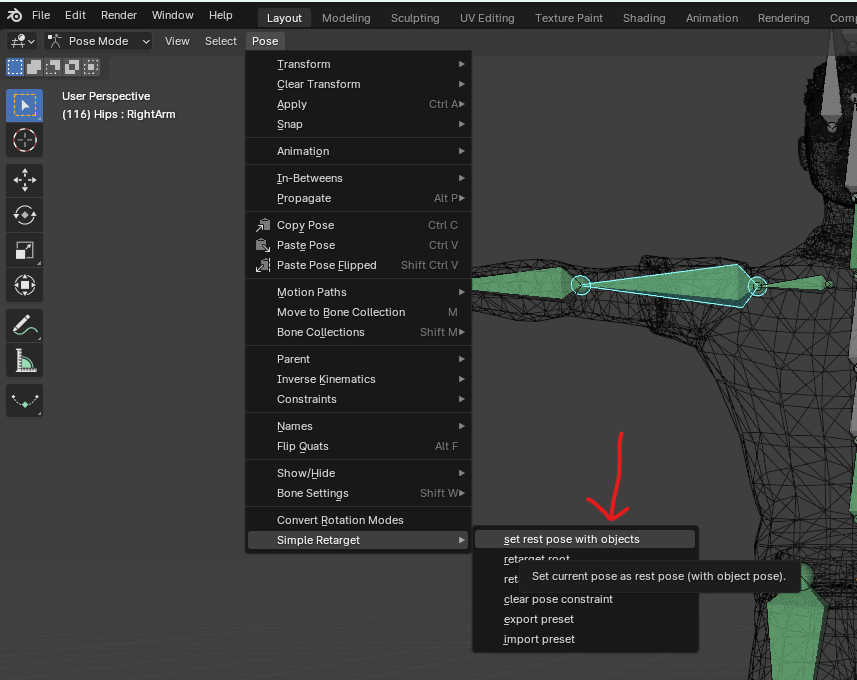
\includegraphics[width=0.5\textwidth]{imgs/restposeQuick.png}
    \caption{Blender Pose Mode - the location of the ``set rest pose with objects" option.}
    \label{fig:restPoseQuick}
\end{figure}

\subsection{Adding bones}
In Object Mode, select the armature. Then go into Edit Mode. With ``Shift+A" we can add a bone.
Select a bone you wish to child to the added bone, then hold shift and select the parent bone. With ``Ctrl+P" we can parent with or without the offset.
You can also extrude bones by selecting a bone and pressing ``e".
Lastly, we can mirror bones to the other side of the avatar. First select the bones to be mirrored in Edit Mode. Then right click and select ``Symmetrize".

\subsubsection{Moving bones}
After adding a bone, we might want to move them into a desired location. In order to do this, we select a joint and press ``g". If we drag the cursor around whilst holding left mouse click, we can see the bone being moved. If it is not moving, you probably still have the ``Snap" option on (see figure \ref{fig:snap}).
\begin{figure}[hbt!]
    \centering
    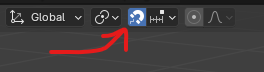
\includegraphics[width=0.5\textwidth]{imgs/snap.png}
    \caption{Blender - the Snap option}
    \label{fig:snap}
\end{figure}

\subsubsection{Weight Painting bones}
To weight paint bones, in Object Mode select the armature, hold control and select the mesh as well. Then with ``Ctrl+Tab" we can select ``Weight Paint". In the Weight Paint mode, we hold alt to select which bone we wish to paint its weights for. If a bone is not added as a Vertex Group, you will not be able to paint for it. I recommend using the wireframe view to paint weights.

When we are done painting one side, we want to copy over the values to ther other side. Use the following link to do this: \href{https://blender.stackexchange.com/a/316052}{\textit{How to mirror existing weight painting from one side to another}}.
For your convenience, here are the steps:
\begin{enumerate}
    \item In Edit Mode, select all of the verticies on side B that you want to update. These verticies will have their weight painting copied from the other side
    \item Switch to weight painting mode.
    \item Enable vertex selection, make sure the verticies are selected, then click Weights $>$ Mirror.
    \item Make sure to select All Groups in the little window that pops up in the bottom left corner.
\end{enumerate}

\paragraph{Auto Weight Painting bones}
In order to automate the process of weight painting, Blender offers us automatic weight painting using bone to vertice distance or envelop. In my experience the first option works better. First select the mesh whilst holding ``shift" then select the armature whilst holding shift. With ``Ctrl+Tab" we can go into weight painting mode. In this mode, press ``a" to select all bones. At the top of the window, we can select the automatic weight painting option (see figure \ref{fig:autoweight}).
\begin{figure}[hbt!]
    \centering
    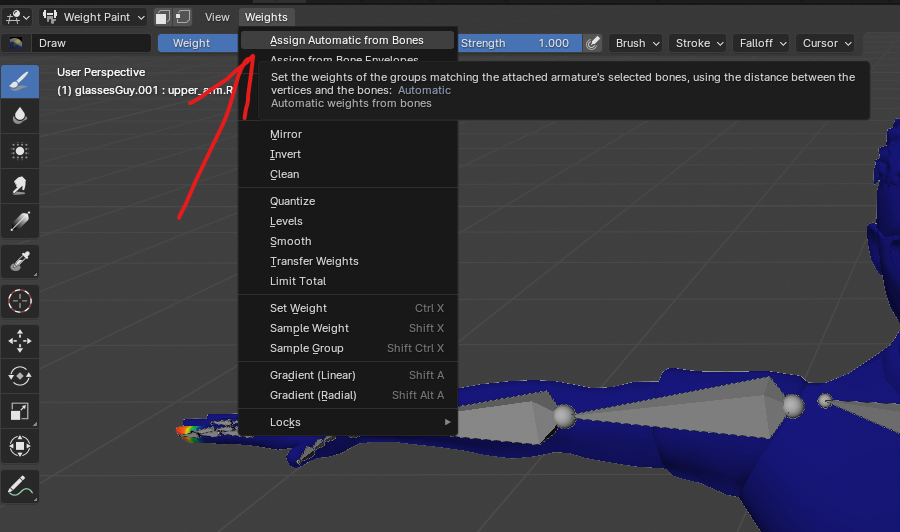
\includegraphics[width=0.5\textwidth]{imgs/autoweightpaint.png}
    \caption{Blender Weight Painting Mode - the automatic weight painting option}
    \label{fig:autoweight}
\end{figure}
Whilst holding ``Alt" we can select individual bones and check if the weight painting worked. In my experience, meshes are often build out of multiple parts (for example clothes and accessories). Because of this, Blender often fails to do the weight painting automatically. A workaround is described in the following post: \href{https://www.reddit.com/r/blenderhelp/comments/hpn4w5/comment/fxuh9l1/?utm_source=share&utm_medium=web3x&utm_name=web3xcss&utm_term=1&utm_content=share_button}{Bone Heat Weighting: failed to find solution for one or more bones}. For your convience, the steps are provided below:
\begin{enumerate}
    \item Select the model, edit mode, select all
    \item CTRL-V - Separate - By Loose Parts
    \item Switch back to object mode. Do NOT deselect anything
    \item Hold shift and select the rig
    \item CTRL-P - Automatic Weights. It'll now work
    \item Shift - deselect the rig. You should now just have the mesh parts selected
    \item CTRL-J to join them back together
\end{enumerate}

\subsection{Automatic weights method 2}
Sometimes the model is too complex for the first method. We need to do something simpler to fix this. Following the guide in \url{https://3dmodels.org/blog/automatic-weights-in-blender/}, we can achieve this by doing the following:
\begin{enumerate}
    \item Check Model/Rig.
    \begin{itemize}
        \item Check scaling: make sure your model and rig aren’t too small – Automatic Weights works best with larger/less dense models.
        \item Check for Overlapping Vertices: overlapping vertices on your model might cause Automatic Weights to fail. To remove them, select all (A) in edit mode, and press M > By Distance to merge them.
        \item Check for Non-Manifold Geometry: check your model for non-manifold geometry such as interior faces and loose vertices – delete these if they’re present.
    \end{itemize}
    \item In Object Mode, select your model first, then select your armature; press Ctrl/Cmd – P to open the parenting menu, and select With Automatic Weights.
\end{enumerate}
Your model should now be attached to your rig! To test it out, try entering Pose Mode by pressing Ctrl/Cmd – Tab and rotating a bone on your armature – if everything worked properly, your mesh should now move in sync with the bones on your armature.

\section{Freemocap - from importing, rigging, to retargeting within Blender}
After recording and exporting with the Freemocap motion capture software. We get a Blender file. Within Blender, we have the ability to import these files, re-rig the Freemocap skeleton to a more common rig like UE Metahuman rig, and finally using the expy plugin, we can retarget the animation onto whatever skeleton we want. This section walks you through these processes.

\subsection{Freemocap - importing and rigging}
Open the .blend file. Make sure you have downloaded and installed the ``Freemocap Adapter Alt" plugin from the \href{https://github.com/ajc27-git/freemocap_tools}{freemocap\_tools} by ajc-27.

Within Object Mode, we can open the adapter menu and go into the ``Add Rig" option (see figure \ref{fig:rigifyfreemocap}). Choose the correct armature, and then add the rig. Now retargeting will become much easier with a more known rig.

After adding the rig, feel free to remove everything else in the hierarchy.
\begin{figure}[hbt!]
    \centering
    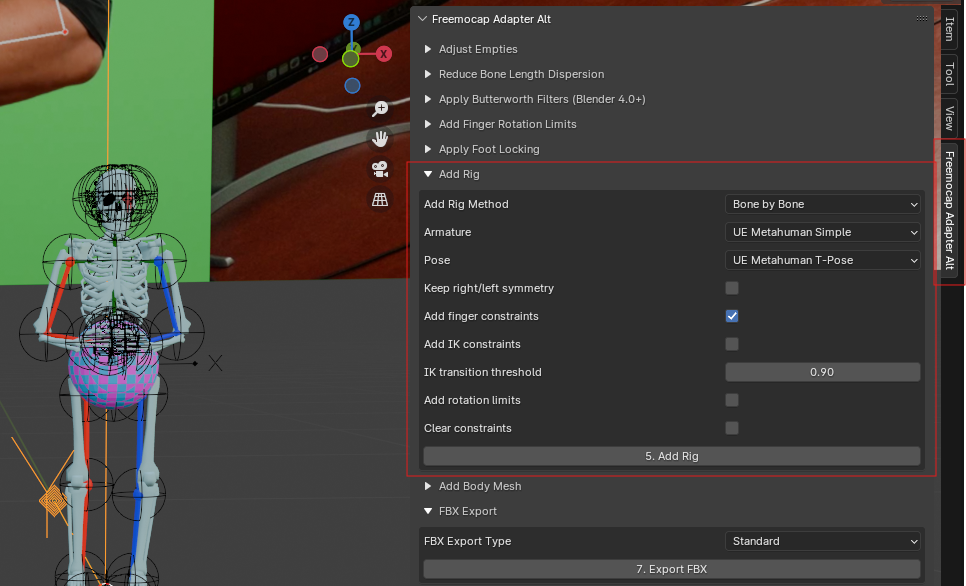
\includegraphics[width=0.8\textwidth]{imgs/rigify.png}
    \caption{Freemocap Adapter Alt - the ``Add Rig" option}
    \label{fig:rigifyfreemocap}
\end{figure}

\subsection{Expy - retargeting freemocap animations}
We will retarget using the \href{https://ballsandninjas.gumroad.com/l/xotibs}{``expy kit"} by balssandninjas. Firstly, import your target avatar (if needed set automatic bone orientation in the import as shown in figure \ref{fig:correctimportsettings}). Make sure to apply all translations to the imported avatar (Object Mode $>$ Object $>$ Apply $>$ All Transforms). Select the target skeleton and go into Pose Mode. Next, open the Expy menu and set the ``Bind To" to the source skeleton root (see figure \ref{fig:retargetexpy}).
After clicking ``Bind Armatures" you can edit the retargeting options in the lower left of the screen.
\begin{figure}[hbt!]
    \centering
    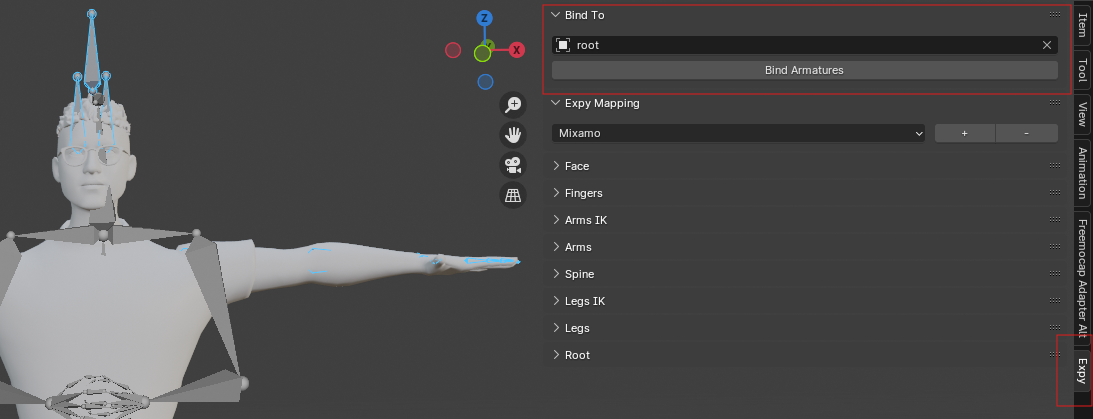
\includegraphics[width=0.8\textwidth]{imgs/retargetExpy.png}
    \caption{Expy kit - the ``Bind To" option}
    \label{fig:retargetexpy}
\end{figure}
\section{StretchSense}\label{section:stretchsense}
\subsection{Pose Matching}
For StretchSense, Pose Matching is also used. On their website, there is a description of how the avatar's pose should be: \url{https://stretchsense.my.site.com/defaulthelpcenter26Sep/s/article/Fidelity-and-SuperSplay-Glove-Unreal-Engine-Streaming}. However, this cannot be done in the Hand Engine software. It is recommended to use software such as Blender, Cinema 4D, Autodesk, etc. The task here is to pose the avatar in a T-pose and provide the following characteristics:
\begin{enumerate}
    \item Hand palms must point directly downwards and be parallel to the ground.
    \item Fingers must be extended, parallel to each other, and aligned along an axis.
    \item Thumbs must be perpendicular to the other fingers, pointing along an axis.
    \item The thumbnail must point towards the body (not always the case).
\end{enumerate}

Sometimes, even after a perfect Pose, the retarget may still produce undesirable results. This is because the target skeleton is different from the source skeleton (different bone lengths and other proportions). To ensure better results, you can adjust the pose (for example, giving pre-rotations to certain bones).

After a meeting with StretchSense we received extra pointers regarding good thumb retargeting. Instead of pointing the thumbnail towards the body, we can try to rotate it in the range of towards the body and fully upwards.


\subsubsection{Exporting and notes on coordinate systems}
Each of the aforementioned software has its own method of importing and exporting avatars. If the final retarget causes the bones to rotate in the wrong directions, it's often because the export from this step didn't go well. Here is further information on why we encounter this specifically for  \textbf{Unreal Engine's coordinate system}.
One of the notable differences between UE and some other 3D software packages or game engines is their choice of coordinate systems and up axis.
In Unreal Engine, the default coordinate system is the "left-handed coordinate system," where the positive X-axis points to the right, the positive Y-axis points forward, and the positive Z-axis points up. This means that the Z-axis is considered the "up" axis in UE.
In most other 3D software packages or game engines, the default coordinate system is the "right-handed coordinate system," where the positive X-axis points to the right, the positive Y-axis points up, and the positive Z-axis points forward. In this coordinate system, the Y-axis is considered the "up" axis.

Because of this difference in the choice of up axis, when importing assets (such as models, animations, or scenes) from other software packages into Unreal Engine, you may encounter issues related to the orientation or alignment of the objects.

When importing into UE, we can give a pre-rotation to the FBX. This can help orient the avatar correctly before inputting it in in UE.
Regardless, we would prefer the export of a skeleton to be correct.

In Blender, we encountered such a problem when trying to retarget to a ReadyPlayerMe avatar. The export settings that helped us at that time are displayed in figure \todo{Use space transform should be off, x forward, z up}
\ref{fig:blenderSettings}.
\begin{figure}[hbt!]
    \centering
    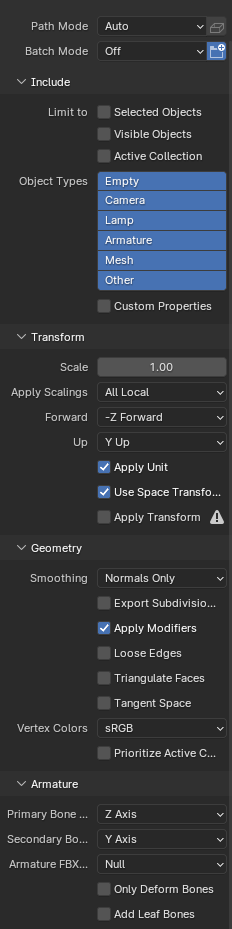
\includegraphics[height=0.9\textheight]{imgs/settings.png}
    \caption{Blender export settings for UE}
    \label{fig:blenderSettings}
\end{figure}

StretchSense has notified us that the coordinate system of Hand Engine is the same as Unreal's coordinate system. In addition, using a good primary bone axis in the export out of Blender is also important. If u see the retarget working in the correct directions, but the mesh of each part are turning in the wrong direction, then you are not using correct bone axis.


%-------------------------------------------------------------------------------
%	REFERENTIES
%-------------------------------------------------------------------------------

\printbibliography

%-------------------------------------------------------------------------------
%	BIJLAGEN 
%-------------------------------------------------------------------------------

%TC:ignore
% \appendix 
% \section{Bijlage {\LaTeX} code}
% Bijgevoegd zijn de \textattachfile{main.tex}{code} en 
% \textattachfile{references.bib}{bibliografie}.
%TC:endignore

%-------------------------------------------------------------------------------
\end{document}